\documentclass[journal]{IEEEtran}

\usepackage[pdftex]{graphicx}
\graphicspath{{img/}}
\usepackage{cite}
\usepackage{amsmath}
\DeclareMathOperator*{\argmin}{arg\,min}
\usepackage{amssymb}
\usepackage{mathtools}
\usepackage{booktabs,siunitx}
\usepackage{threeparttable}
%\usepackage{subcaption}
\usepackage{multirow}
\usepackage[caption=false,font=footnotesize,labelfont=sf,textfont=sf]{subfig}

%\usepackage{endfloat}

% TODO: remove
	\usepackage{xcolor}
	\newcommand\TODO[1]{\textcolor{red}{TODO: #1}}
	\newcommand\FIXME[1]{\textcolor{blue}{FIXME: #1}}

\begin{document}
\title{Title of the Paper}


\author{Michael~Rebsamen,
        Jan~Riedo,
        Michael~Mueller% <-this % stops a space
\thanks{Biomedical Engineering, University of Bern}% <-this % stops a space
\thanks{Authors e-Mail: michael.mueller4@students.unibe.ch, jan.riedo@students.unibe.ch, michael.rebsamen@students.unibe.ch}}% <-this % stops a space
\markboth{Biomedical Engineering, Medical Image Analysis Lab, \today}%
{Title of the Paper}
\maketitle

\begin{abstract}
Machine learning (ML), white matter (WM), grey matter (GM), cerebrospinal fluid (CSF), background (BG)
\end{abstract}
\begin{IEEEkeywords}
MRI, Segmentation, Machine Learning, DF, kNN, SVM
\end{IEEEkeywords}


\section{Introduction}
Segmentation of brain tissues from magnetic resonance images (MRI) has many clinical applications. Clinicians gain useful information from a separation of tissue into its three main anatomical types: white matter, grey matter, and cerebrospinal fluid. Voxel-based morphometric measures have been used to investigate brain disorders like Alzheimer’s disease~\cite{busatto2003voxel}, Parkinson's disease~\cite{price2004voxel} or temporal lobe epilepsy~\cite{rummel2017personalized}. However, manual segmentation of MRI is a labour-intensive task requiring expert skills. Fully automatic approaches for brain tissue segmentation are therefore a topic of active research. A good algorithm classifies the tissue types with high accuracy across a variety of images from different patients. Such a classification is a typical task for machine learning. These algorithms tend to perform well given enough training data during the learning phase. The availability of ground-truth data in sufficient quantity and quality for supervised learning is a particular challenge when working with medical images due to privacy concerns and the costs for manual segmentation. Optimization of the learning phase with a limited number of training data is therefore required.

Current research is evaluating a variety of different discriminative machine learning algorithms on the classification task of brain segmentation. Most proposed methods use ensembles such as Decision Forests (DFs), with several individual machine learning algorithms combined or sequentially applied. A classic DF implementation was performed by Yaqub et al. \cite{Yaqub2014} with results matching current benchmark in brain segmentation. Many extensions to Df with probabilistic models were successfully tested such as conditional random fields \cite{Pereira2016}. However, it was shown that even the simple, instance based k-nearest neighbors (kNN) algoritm yields accurate results \cite{Anbeek2004,Cocosco2003,Warfield2000} for brain tissue classification. Furthermore, linear classifiers under convex loss functions such as (linear) Support Vector Machines (SVMs) were successfully applied for automatic brain tumor segmentation \cite{Bauer2011}. Another approach of this type of algorithms is the Stochastic Gradient Descent (SGD) which is well established in solving of optimization problems and a standard for training artificial neural networks \cite{LeCun1998}. It gained importance in the field of large-scale machine learning problems \cite{Bottou2010}. There is no record so far about an application of mere SGD on brain segmentation. Current development has the tendency to bring more accurate results by incorporating 3D neighborhood information \cite{Li2011,Despotovic2013}, prior information from atlases\cite{Pohl2006,Ashburner2005}, deformable models \cite{Moreno2014} or combinations thereof \cite{Ortiz2014}.

In this experiment, we compare the performance of four well known machine learning algorithms by means of accuracy, computational efficiency, and amount of training data required. We use the existing medical image analysis pipeline to assess the following supervised learning algorithms: decision forest (DF), k-nearest neighbours (kNN), support vector machine (SVM), and stochastic gradient descent (SGD). The algorithms are trained using seven features extracted from a set of 70 MRI and the prediction of the segmentation is evaluated on a different set of 30 MRI. All algorithms were able to classify the brain tissue types, although with different accuracy and runtime behaviour. Unsurprisingly, the highest dice coefficient is achieved by combining the predictions of all four algorithms to an ensemble and by using all features. An analysis of the feature importance reveals a different influence of the features types between the algorithms.


\section{Methods}

\subsection{Dataset}
All experiments were conducted on a subset of 100 unrelated, healthy subjects from a dataset provided by the \textit{Human Connectome Project} \cite{van2013wu}. From each individual, a total of eight 3-tesla head MRI are available: T1 and T2-weighted image volumes not skull-stripped (but defaced for anonymization) and skull-stripped with a bias field correction, and both modalities once in native T1 space and once in MNI-atlas space \cite{mazziotta2001probabilistic}.

Ground-truth labels are automatically generated using \textit{FreeSurf}, assigning each voxel either to background, white matter, grey matter, or cerebrospinal fluid. The dataset was split in a training set with 70 images and a test set with 30 images.

\subsection{Pipeline}

Training and testing data are loaded sequentially, each put through the pipeline consisting of: registration, pre-processing, feature extraction and ML training/classification. For testing, two additional steps, namely post-processing and evaluation are added.

The data was registered to an atlas with a multi-modal rigid transformation using a regular step gradient descent optimizer. Skull stripping and bias field correction were applied in order to have images of the brain only, with less influence of the MRI scanning characteristics. Furthermore, the preprocessing module applis a gradient anisotropic diffusion filter and z-score normalization.

Preprocessed data is then fed into the feature extraction module, where seven features are computed. The feature matrix consists of three coordinate features, a T1 and a T2 intensity feature, and a T1 and T2 gradient feature. During feature extraction, a random mask is applied in order to randomly select a fraction of the voxels available. The mask is adjustable individually for BG, WM, GM, and CSF. This is where the pathways of training and testing split up: training data is lastly fed to a certain supervised machine learning algorithm for training, whereas the testing data is classified with the previously created model. The classified testing data is then forwarded to a post-processing module where a dense conditional random field \cite{krahenbuhl2011efficient} is applied.
Finally, the classification is evaluated based on a comparison with the ground truth, where a dice coefficient is computed (see chap.~\ref{ch.eval}).


\FIXME{The medical image analysis pipeline consists of seven phases. In the pre-processing phase, an intensity normalization is performed on the images to ensure comparable grey scale ranges among all images in the subsequent steps. Similarly, the registration phase registers the images to an atlas space to establish a common coordinate system. In the feature extraction phase, seven features are calculated for each voxel: three coordinates corresponding to the position of the voxel in the atlas space, and an intensity and a gradient on both the T1 and T2 modalities. A subset of voxels is choosen randomly to be used for training. During the learning phase, the selected algorithm is trained to classify voxels based on the given features. In the segmentation phase, the trained algorithm is used to classify all voxels in previously unseen test images. The post-processing phase aims to reduce noise by eliminating small isolated regions with a dense conditional random field \cite{krahenbuhl2011efficient}. Finally, the evaluation phase assesses the performance of the segmentation by comparing the result to ground-truth and calculating a dice coefficient for each class.}\\\\

\FIXME{Jan's suggestion:}\\
Training and testing data are loaded sequentially, each put through the pipeline consisting of: registration, pre-processing, feature extraction and ML training/classification. For testing, two additional steps, namely post-processing and evaluation are added.\\
The data was registered to an atlas space with a multi-modal rigid transformation, using a regular step gradient descent optimizer to establish a common coordinate system. Skull stripping and bias field correction were applied in order to have images of the brain only, with less influence of the MRI scanning characteristics. Furthermore, the preprocessing module applies a gradient anisotropic diffusion filter and z-score normalization to ensure comparable grey scale ranges among all images in the subsequent steps.\\
Preprocessed data is then fed into the feature extraction module, where seven features are computed. The feurate matrix consists of three coordinate features corresponding to the position of the voxel in the atlas space, and an intensity and a gradient on both the T1 and T2 modalities. During feature extraction, a random mask is applied on the training data in order to randomly select a subset of the voxels available. The mask is adjustable individually for BG, WM, GM, and CSF. During the learning phase, the selected algorithm is trained to classify voxels based on the given features. In the segmentation phase, the trained algorithm is used to classify all voxels in previously unseen test images. The classified testing data is then forwarded to a post-processing module where a dense conditional random field \cite{krahenbuhl2011efficient} aims to reduce noise by eliminating small isolated regions. Finally, the evaluation phase assesses the performance of the segmentation by comparing the result to ground-truth and calculating a dice coefficient (see sec.~\ref{ch.eval}) for each class.\\\\


\subsection{Decision Forest (DF)}
\TODO{MM: \textbf{Short} intro to DF, ref to \ref{f.df_gridsearch}}

\subsection{k-Nearest Neighbors (kNN)}
The k-Nearest Neighbors algorithm does not construct a general model, however stores instances of the training data. A query point is assigned to a certain class based on the votes, which come from the nearest neighbors of the point. A weight function assigns a weight which is inverse proportional to its distance to the point. The characteristics of kNN lead to a relatively low training time, and a rather high computation time for new points, depending on the amount of neighbors defined to vote. A hyperparameter search was conducted for the k-value. The higher k, the better the overall dice with the drawback of a higher computation time. A value of $k=20$ was found to be fast with only little trade-off in computation time.

\subsection{Support Vector Machine (SVM)}
Classification using Support Vector Machines (SVM) tries to find a hyperplane separating the data in a high-dimensional feature space. Given the feature vector $x_i$ and the binary label $y_i$, the SVM solves the following optimization problem during training:
\begin{equation}
\begin{split}
\min_{w, b, \xi} \ & \frac{1}{2}w^Tw + C\sum_{i=1}^m \xi_i \\
\ \text{ s.t. } & y_i(w^T\phi(x_i)+b) \geq 1-\xi_i, \; i = 1, \ldots, m \\
& \xi_i \geq 0, \; i = 1, \ldots, m
\end{split}
\end{equation}
where $w\in \mathbb{R}^n $ is the normal vector and $b \in \mathbb{R}$ the offset of the separating hyperplane and $\phi(x_i)$ maps $x_i$ into a higher-dimensional space.

The SVM implementation is based on libSVM \cite{chang2011libsvm}. Multiclass classification is solved with a \textit{one-against-one} approach. To output probabilities, the predictions are calibrated using \textit{Platt} scaling in which multiclass problems require an additional cross-validation which is an expensive operation for large datasets.

Given the relative low number of available features, we have chosen a radial basis function (RBF) kernel. A regularization term $C$ and a model capacity $\gamma$ needs to be chosen. These hyperparameters were determined with an exhaustive search and cross-validated on a subset of the training data, yielding $C=500$ and $\gamma=0.00005$.

\subsection{Stochastic Gradient Descent (SGD)}
Stochastic Gradient Descent (SGD) is widely used in machine learning for solving optimization problems iteratively. SGD has proven to be efficient for large-scale linear predictions \cite{zhang2004solving}.

In the current context, SGD learns a linear scoring function $f(x) = w^Tx + b$ with model parameters $w$ and $b$ by minimizing the training error
\begin{equation}
\argmin_{w,b} \frac{1}{m}\sum_{i=1}^mL(y_i, f(x_i)) + \alpha R(w)
\end{equation}
where $L$ is a loss function that measures miss-classifications, $R$ is a regularization term penalising model complexity, and $\alpha$ is a non-negative hyperparameter.

In each iteration, a sample is randomly chosen from the training set and the model parameters are updated according
\begin{equation}
w \leftarrow w - \eta \left(\alpha \frac{\partial R(w)}{\partial w} + \frac{\partial L (w^Tx_i + b, y_i)}{\partial w} \right)
\end{equation}
where $\eta$ is the learning rate controlling the step size.

We use a smoothed hinge loss (\textit{modified\_huber}) for the loss function $L$, a $l_2$ penalty ($||w||_2$) for the regularization term $R$, and a gradually decaying learning rate. This makes SGD similar to a linear SVM. Again, the hyperparameters $\eta = 0.5$ and $\alpha = 0.01$ were determined with an exhaustive search and cross-validated on a subset of the training data.


\subsection{Performance Evaluation}\label{ch.eval}
The Dice coefficient is a commonly used metric to compare the spatial overlap, ranging from 0 (no overlap) to 1 (perfect overlap). To evaluate the accuracy of the segmentation, a Dice coefficient is calculated between the prediction (E) and ground-truth (G) for each of the three labels. 
\begin{equation}
D = \frac{2|E \bigcap G|}{|E| + |G|} = \frac{2 TP}{2 TP + FP + FN}
\end{equation}

\section{Results}
\subsection{Segmentation Accuracy}
\TODO{MR: table and boxplot}
All algorithms tested and optimized were able to yield a good result for brain segmentation. The performance measured with the dice coefficient can be found in Tab.~(\ref{tab:perf_compare}). Comparisons of computation time can be seen in Tab.~(\ref{tab:time_compare}).\\

\subsection{Runtime}
\TODO{MR: barplot}

\subsection{Feature Inspection}

%Feature selection is another key part of the machine learning process. Features are also called variable or attribute and describe the model. Irrelevant and redundant features do not contribute to the accuracy of the predictive model, at worst they decrease the accuracy. The used feature set consists of seven features, f1-f3: Coordinate features, f4: T1 intensity, f5: T1 gradient, f6: T2 intensity, f7: T2 gradient. 


The following Fig~(\ref{scatterplot}) shows the scatter matrix of all the features. The whole dataset of 100 images was used for this evaluation. On the diagonal are the histograms to visualize the data distribution of each feature. The first three histograms are of the coordinate features and are normally distributed. The fifth and sixth histograms belong to the intensity features and follow a non normal distribution. The last two histograms are of the gradient features and are half normal distributed. The right upper part of the diagonal visualizes the linear correlation between each of the feature with the associated correlation coefficient. The left bottom part of the diagonal is redundant to the upper part. 

The coordinate features with an correlation coefficient between -0.11 and 0.05 are independent and do not correlate with any other feature at all. The first intensity feature has a moderate linear relationship with the second intensity feature and a weak with the first gradient feature. The second intensity feature has also a moderate correlation with both of gradient features. The gradient features correlate with an correlation coefficient of 0.82 very strong among themselves.    

\TODO{Change label in ScatterMatrixPlot, Mike}

\begin{figure}[h]
	\centering
	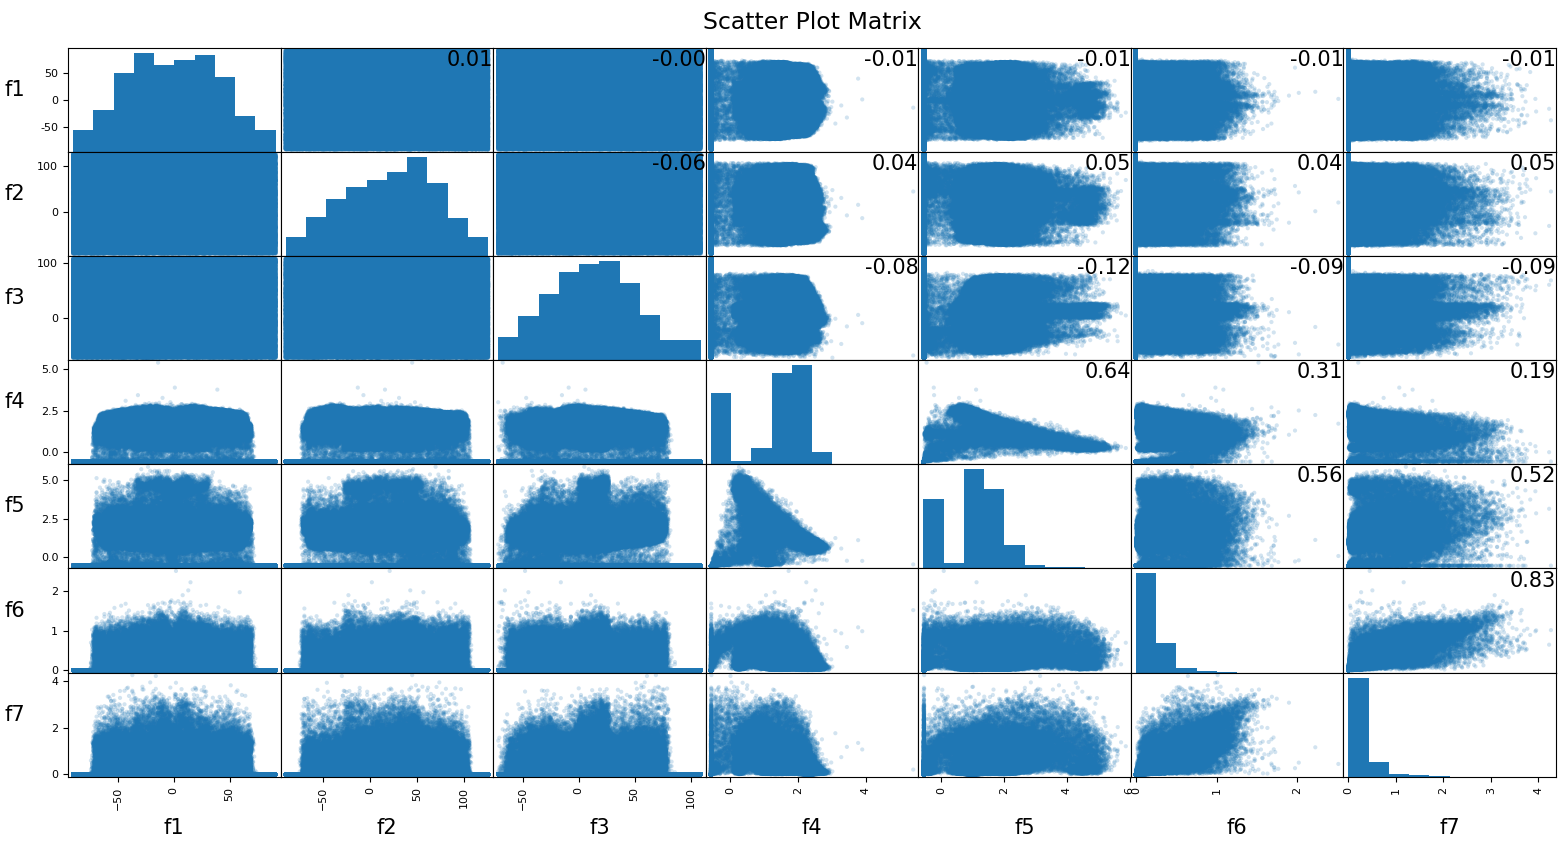
\includegraphics[width=0.49\textwidth]{images/ScatterPlotMatrix}
	\caption{Scatter plot of the features with correlation coefficient}
	\label{scatterplot}
\end{figure}

The following Fig~(\ref{FeatEval}) visualizes the influence of each feature type and the used algorithms. The feature types are divided in three coordinate, two intensity and two gradient features. The first column in this figure is calculated with all the features combined and is considered as a reference. Each column belongs to a single feature type in which the dice of the four used algorithms is visualized. Vertically in line is each dice for the gray matter, white matter and the cerebrospinal fluid disposed.

\TODO{Describe the plot, insert Legend of W, V or C? in figure 3, Mike}
\begin{figure}[h]
	\centering
	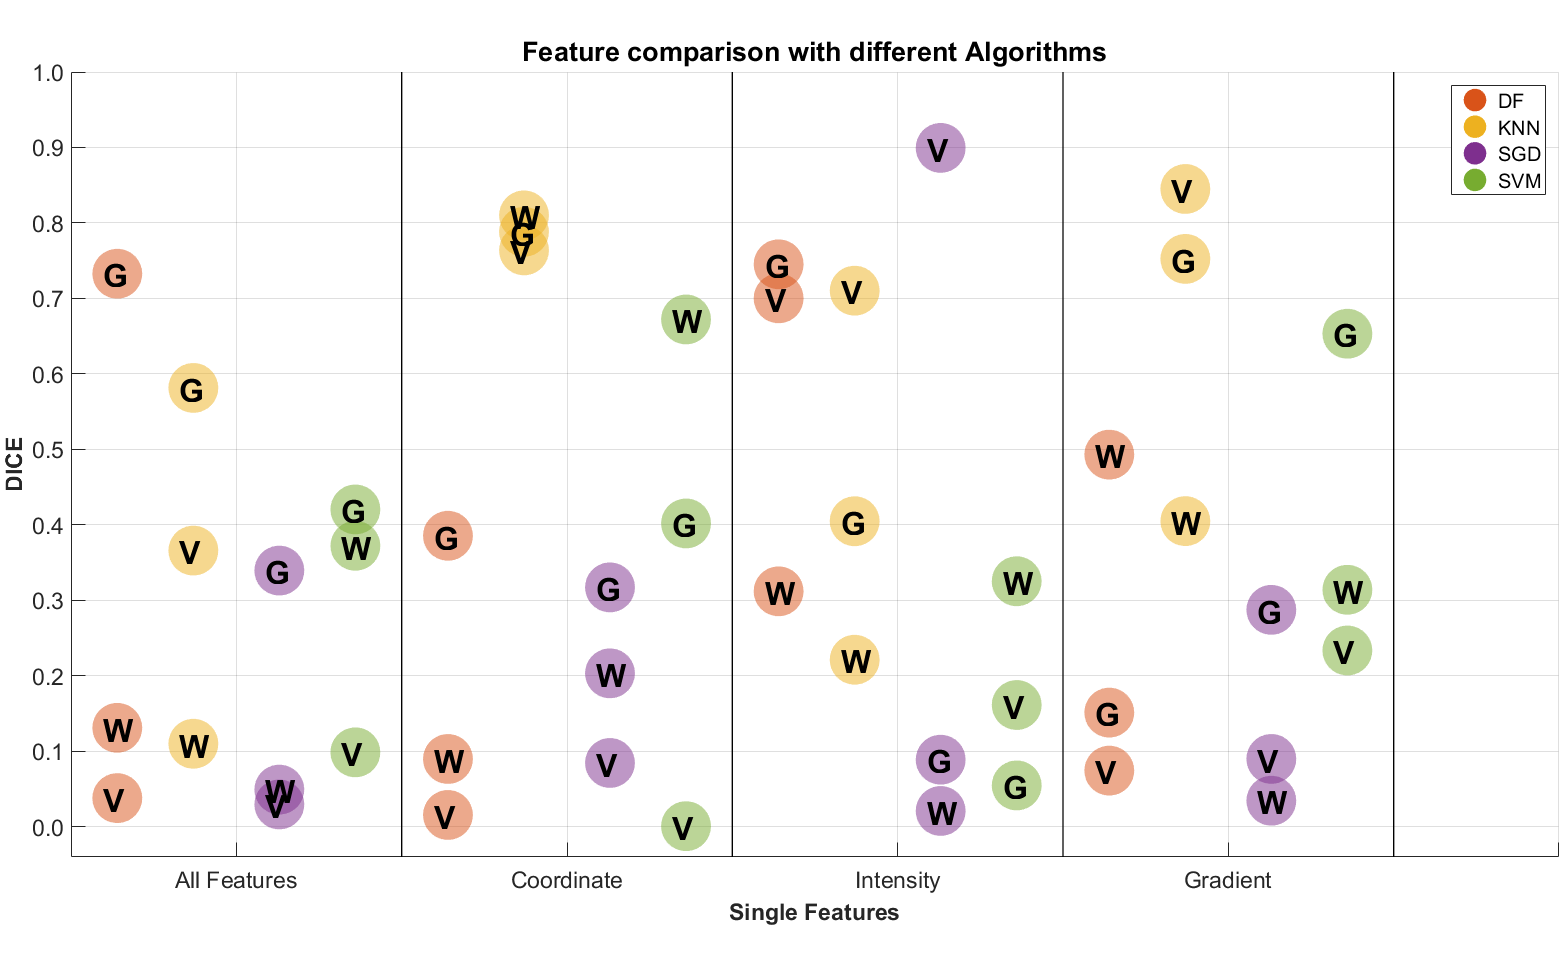
\includegraphics[width=0.49\textwidth]{images/FeatureEvaluation}
	\caption{Feature evaluation of single features with different algorithms, preprocessed.}
	\label{FeatEval}
\end{figure}



\subsection{Ground Truth Validity}
\TODO{JR: part in discussion?}

The importance of looking at the images and not only at the numbers shall be presented based on one example MRI image, segmented with kNN. In Fig.~(\ref{f.ground_truth}) we see one slice of a brain, segmented in three different ways. On the left, we see a kNN segmentation based on non-coordinate features. The one in the middle is segmented with kNN based on all features. On the right we see the ground truth. Although the middle image shows a substantially better result in CSF dice than the left (0.68 vs. 0.76) we can barely see an improved CSF segmentation with bare eyes. What we see however, is a big difference on how detailed the white and grey matter are segmented, thus leading to a better overall segmentation. Another fact which shall be presented here is that the ground truth image is not a real ground truth. It is an image segmented by another algorithm. In Fig~(\ref{f.knn_a}) a better segmentation of the center part (white matter) is achieved compared to the ground truth image in Fig~(\ref{f.knn_c}) (background).

\begin{figure}
	\centering
	\subfloat[]{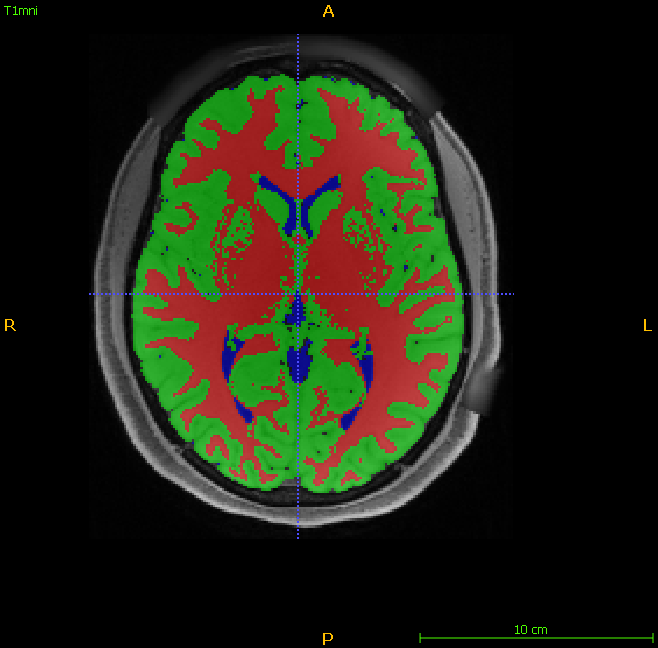
\includegraphics[width=0.3\linewidth]{images/knn_no_coord}\label{f.knn_a}}
	\hfill
	\subfloat[]{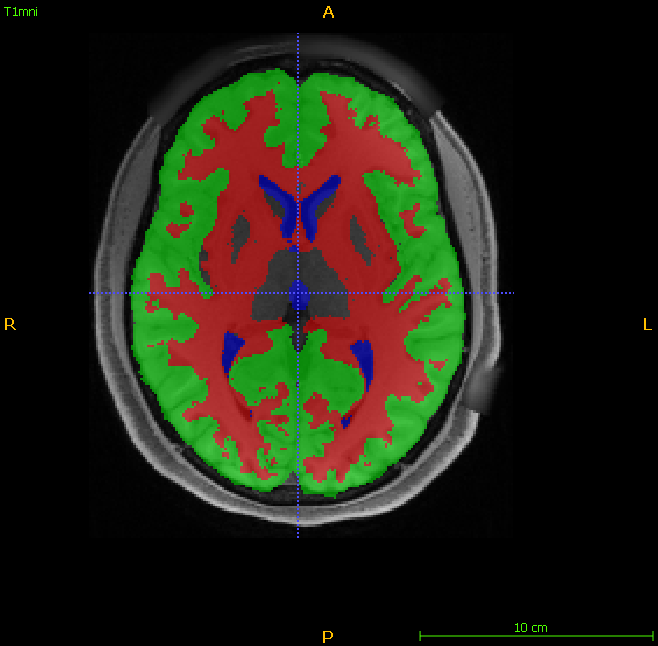
\includegraphics[width=0.3\linewidth]{images/knn_all}}
	\hfill
	\subfloat[]{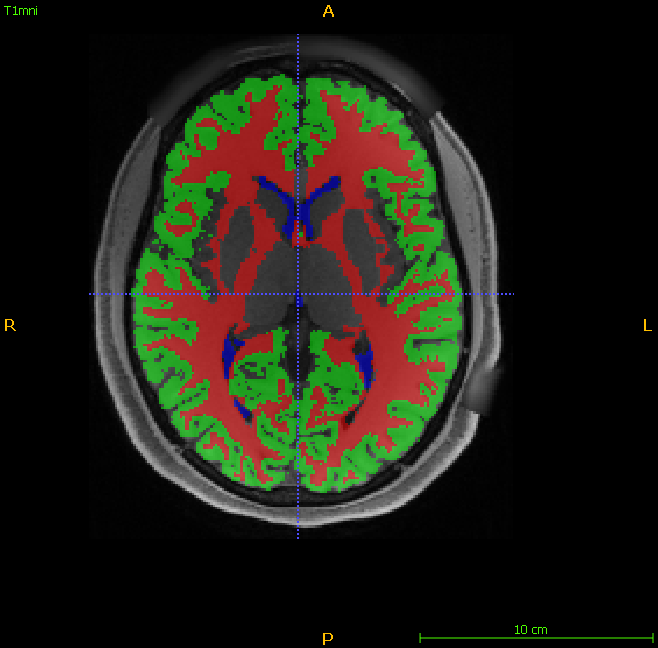
\includegraphics[width=0.3\linewidth]{images/knn_ground_truth}\label{f.knn_c}}
	\caption{(a) kNN segmented image based on non-coordinate features with dice values 0.86/0.82/0.68. (b) kNN segmented image based on all features with dice values 0.80/0.79/0.76. (c) Ground truth.}
	\label{f.ground_truth}
\end{figure}



\subsection{Random Mask Optimization}

One major task to handle was the low value for the CSF. Dice values above 0.5 were hard to achieve. One way to improve the dice for CSF was to optimize the random mask with respect to the fraction of CSF voxels taken into account. The effects of the random mask on the CSF dice can be seen in Fig.~(\ref{f.random_mask}). Best results were achieved with a fraction of 0.004 CSF, approximately the same fraction as for white matter and grey matter. All following results are based on this optimized mask.
\begin{figure}[h!]
	\centering
	\subfloat[]{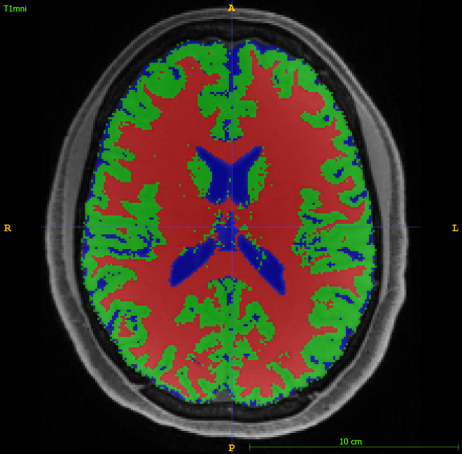
\includegraphics[width=0.3\linewidth]{images/ven_0_4}}
	\hfill
	\subfloat[]{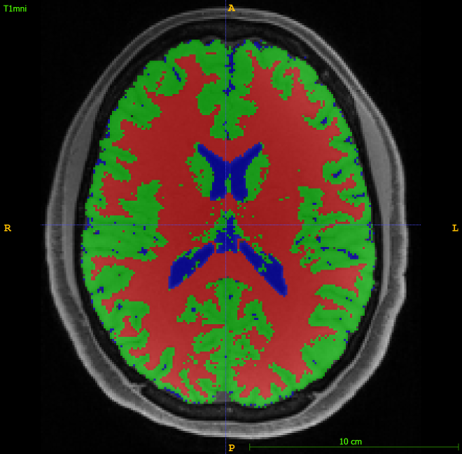
\includegraphics[width=0.3\linewidth]{images/ven_0_04}}
	\hfill
	\subfloat[]{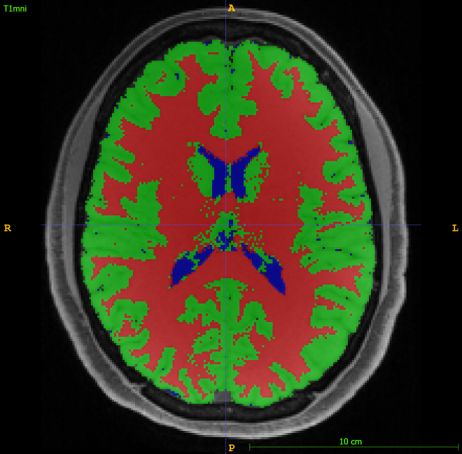
\includegraphics[width=0.3\linewidth]{images/ven_0_004}}
	\caption{Optimization of the random mask parameter for CSF. Fraction of CSF voxels taken into account $f_v$ and dice value for this certain parameter $d_v$ are: ($f_v$ / $d_v$) (a) 0.4 / 0.22, (b) 0.04 / 0.44, and (c) 0.004 / 0.62.}
	\label{f.random_mask}
\end{figure}


\subsection{Algorithm Performance}
\TODO{MR: in A and B}



The decision forest algorithm was enhanced with normalized features, a higher number of CSF voxels in the training set and the optimization of the hyperparameters (see Fig.~\ref{f.df_gridsearch}). With this settings, the max dice coefficient was lifted from 0.703 to 0.754. This result was achieved with 80 trees and 3000 max nodes.

\begin{figure}[h!]\label{f.df_gridsearch}
	\centering
	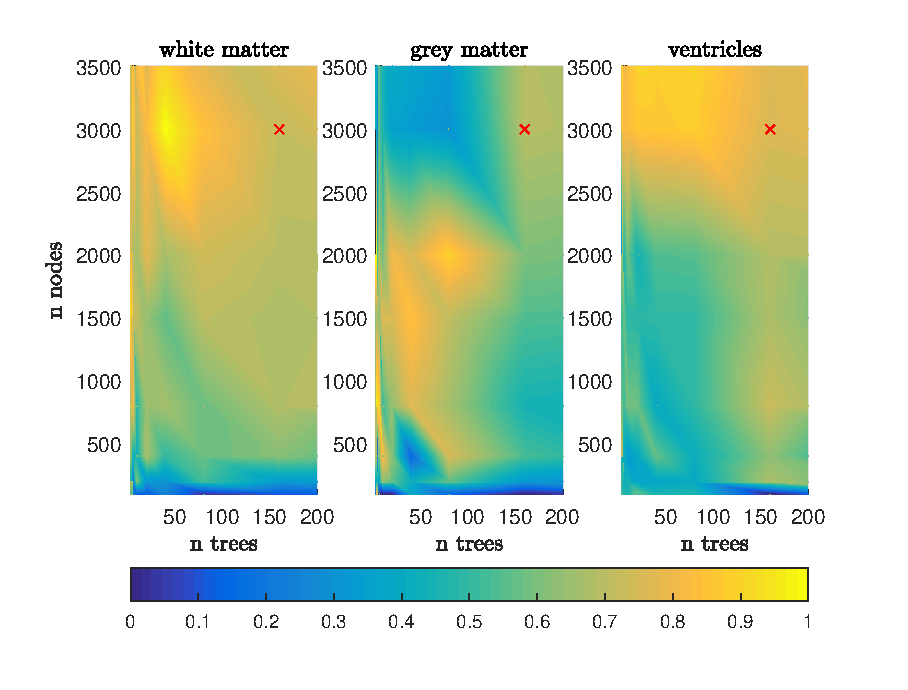
\includegraphics[width=0.48\textwidth]{images/df_grid}
	\caption{DF plot of grid search for white matter, grey matter and cerebrospinal fluid. The red cross marks the chosen hyperparameters number of trees~=~160 and maximum nodes per tree~=~3000. Color does not represent dice, the data is stretched individually for all three plots.}
\end{figure}



Statistical distribution of the dice coefficients can be seen in Fig. \ref{f.boxplot}. DF and SVM achieve a similar mean dice score but SVM has a lower variance for CSF.
\begin{figure}\label{f.boxplot}
	\centering
	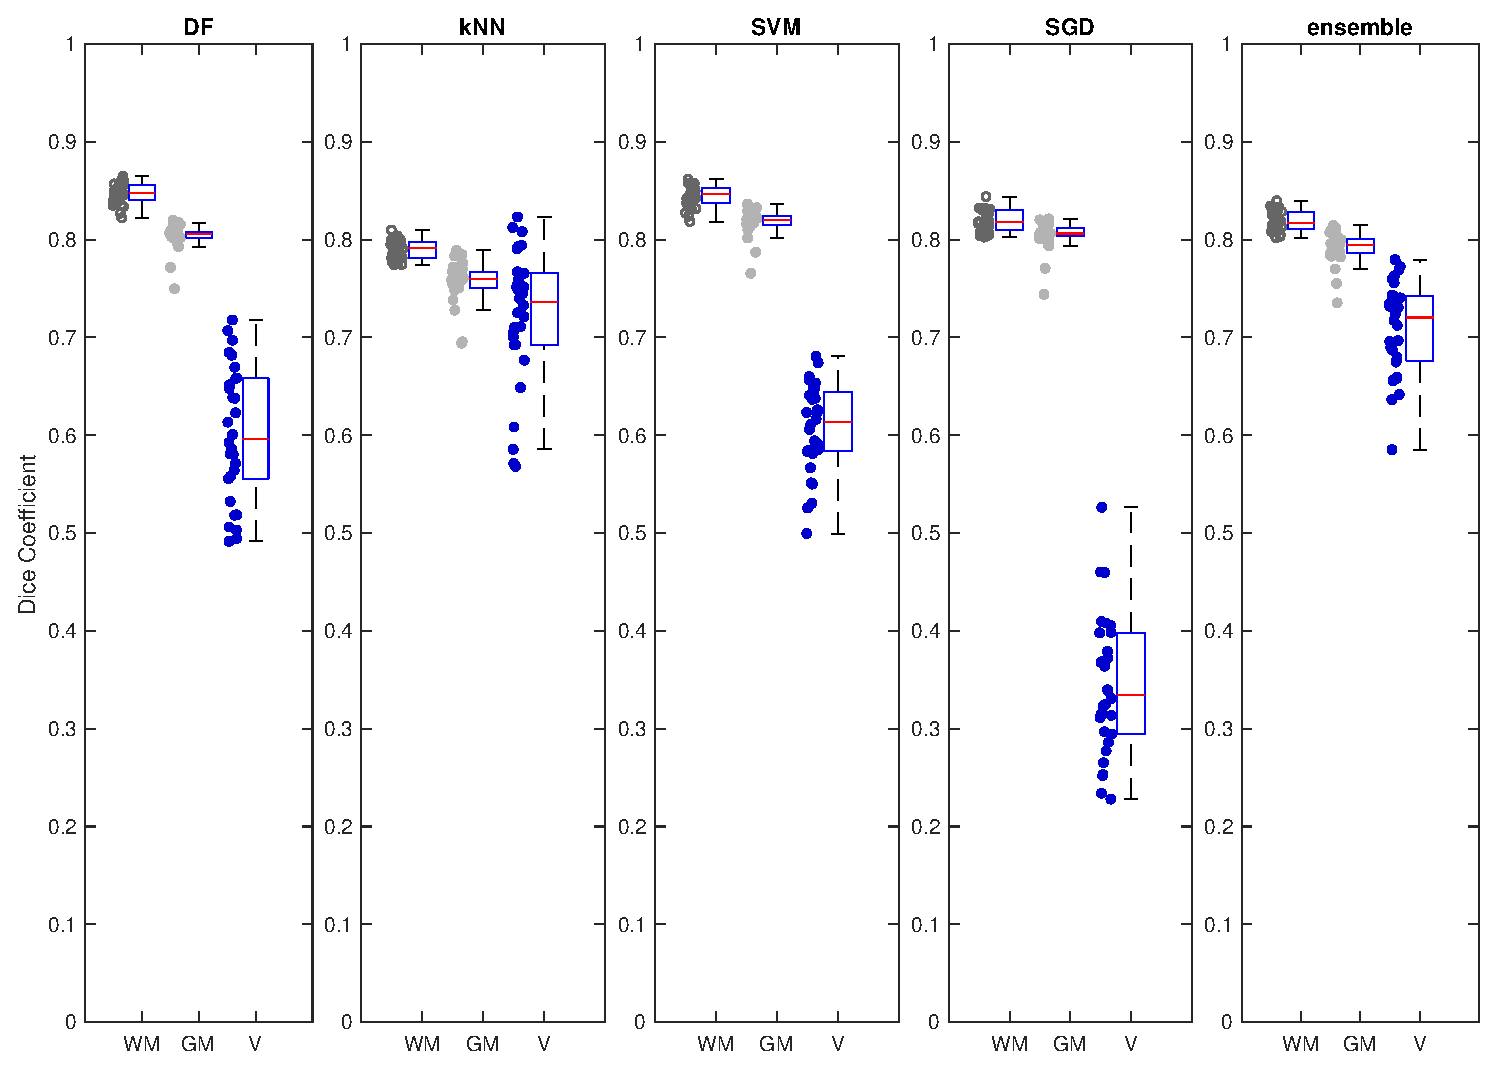
\includegraphics[width=0.48\textwidth]{images/boxplot}
	\caption{Distribution of dice coefficients with optimal hyper-parameters for each algorithm on the full training set of 70 images.}
\end{figure}

Comparison of computation time for training and testing is shown in Fig. \ref{f.runtimebarplot}.
\begin{figure}\label{f.runtimebarplot}
	\centering
	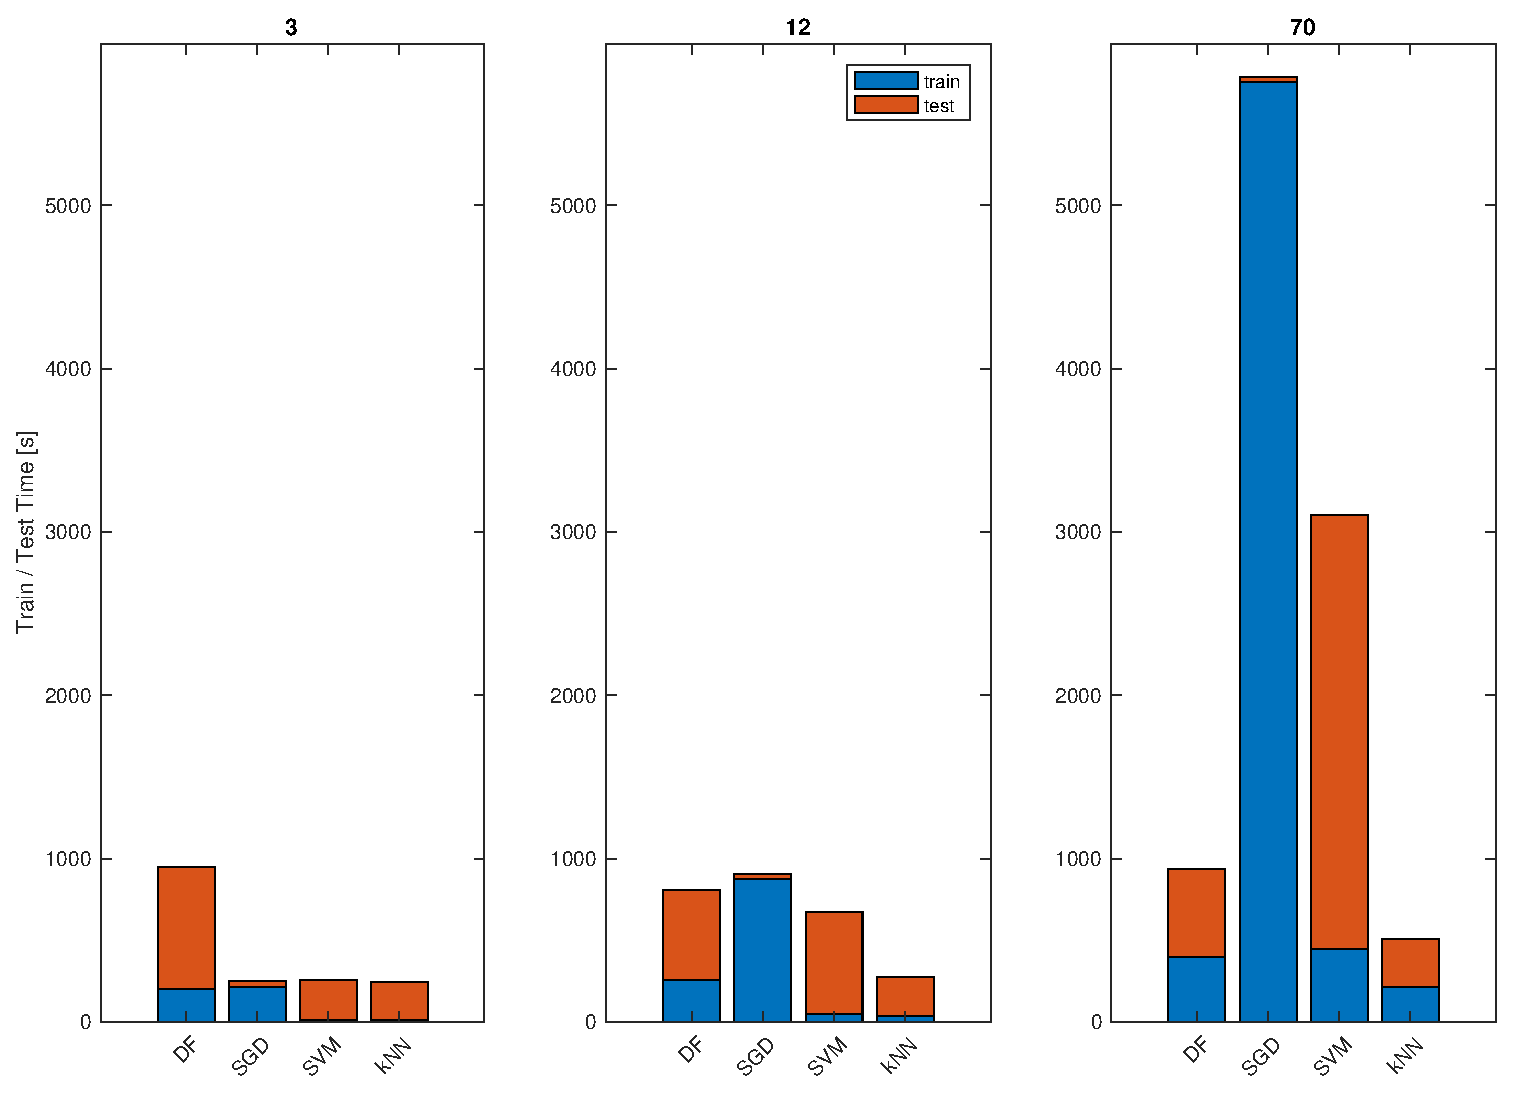
\includegraphics[width=0.48\textwidth]{images/runtimes}
	\caption{Time for training and testing of the algorithms with training set sizes of 3, 12 and 70 samples. Test time is for one sample.}
\end{figure}


\begin{table*}[t]
\renewcommand{\arraystretch}{1.2}
\newcommand\mulrow[2]{\multirow{#1}{*}{\shortstack[c]{#2}}}
\caption{Performance Comparison of ML Algorithms}
\label{tab:perf_compare}
\centering
\begin{threeparttable}
\begin{tabular*}{0.9\textwidth}{@{\extracolsep{\fill}}c*{6}{S[table-number-alignment=center,table-figures-decimal=2,table-auto-round]}@{}}
\toprule
Features & {Size Dataset} & {\shortstack[c]{DF}} & {\shortstack[c]{kNN}} & {\shortstack[c]{SVM}} & {\shortstack[c]{SGD}} & {\shortstack[c]{ensemble}}\\
\midrule
\mulrow{3}{All\\(f1-f7)}
	& 3		&	{0.85/0.81/0.62} 	& {0.70/0.57/0.50}	& {0.83/0.80/0.61}	& {0.82/0.80/0.35}	& {-}\\
	& 12	&	{0.85/0.81/0.59}			& {0.75/0.66/0.67}	& {0.84/0.81/0.61}	& {0.82/0.80/0.34}	& {-}\\
	& 70	&	{0.85/0.80/0.60}			& {0.80/0.76/0.72}	& {0.84/0.82/0.61}	& {0.82/0.80/0.34}	& {0.82/0.79/0.71}\\
\midrule
\mulrow{3}{Coordinates only\\(f1-f3)}
	& 3		&	{0.67/0.63/0.22}		& {0.70/0.55/0.41}	& {0.59/0.52/0.0}	& {0.17/0.23/0.00}	& {-}\\
	& 12	&	{0.67/0.64/0.11}			& {0.74/0.63/0.56}	& {0.59/0.57/0.0}	& {0.19/0.22/0.00}	& {-}\\
	& 70	&	{0.67/0.64/0.16}			& {0.77/0.71/0.62}	& {0.60/0.58/0.31}	& {0.17/0.21/0.00}	& {-}\\
\midrule
\mulrow{3}{All non-coordinates \\(f4-f7)}
	& 3		&	{0.84/0.80/0.50}		& {0.85/0.80/0.45}	& {0.84/0.79/0.0}	& {0.82/0.80/0.34}	& {-}\\
	& 12	&	{0.85/0.80/0.49}			& {0.85/0.81/0.45}	& {0.85/0.80/0.45}	& {0.82/0.80/0.33}	& {-}\\
	& 70	&	{0.85/0.80/0.48}			& {0.85/0.81/0.54}	& {0.85/0.80/0.44}	& {0.82/0.80/0.34}	& {-}\\
\bottomrule
\end{tabular*}
\begin{tablenotes}
\item Overview of achieved accuracy for the different algorithms. Mean dice scores for white matter/grey matter/cerebrospinal fluid.
\item f1-f3: Coordinate features, f4: T1 intensity, f5: T1 gradient, f6: T2 intensity, f7: T2 gradient.
\end{tablenotes}
\end{threeparttable}
\end{table*}

\begin{table*}[t]
\renewcommand{\arraystretch}{1.2}
\newcommand\mulrow[2]{\multirow{#1}{*}{\shortstack[c]{#2}}}
\caption{Runtime}
\label{tab:time_compare}
\centering
\begin{threeparttable}
\begin{tabular*}{0.9\textwidth}{@{\extracolsep{\fill}}c*{6}{S[table-number-alignment=center,table-figures-decimal=2,table-auto-round]}@{}}
\toprule
Features & {Size Dataset} & {\shortstack[c]{DF}} & {\shortstack[c]{kNN}} & {\shortstack[c]{SGD}} & {\shortstack[c]{SVM}}\\
\midrule
\mulrow{3}{All\\(f1-f7)}
	& 3		&	{205.4/22310.2}	& {13.4/7023.7}	& {214.9/1219.6}	& {15.1/7289.7}\\
	& 12		&	{258.7/16563.6}	& {38.1/7090.0}	& {259.9/1250.0}	& {48.2/18730.5}\\
	& 70		&	{401.4/16116.2}	& {215.5/8873.5}	& {445.3/1279.6}	& {448.1/79668.4}\\
\midrule
\mulrow{3}{Coordinates only\\(f1-f3)}
	& 3		&	{-}	& {10.4/4391.5}	 	& {-}	& {15.4/12178.7}\\
	& 12	&	{-}	& {34.7/5449.3}		& {-}	& {62.2/43404.3}\\
	& 70	&	{-}	& {196.4/6112.8}	& {-}	& {957.9/221440.5}\\
\midrule
\mulrow{3}{All non-coordinates \\(f4-f7)}
	& 3		&	{-}		&	{10.1/10084.7}	& {-}	& {12.4/6647.9}\\
	& 12	&	{-}		&	{34.6/18768.6}	& {-}	& {39.8/18691.1}\\
	& 70	&	{-}		&	{194.2/16555.7}	& {-}	& {323.2/80532.7}\\
\bottomrule
\end{tabular*}
\begin{tablenotes}
\item \FIXME{Overview of the computation time in seconds for all algorithms (training time/testing time). Computation time includes pre- and post-processing.}
\end{tablenotes}
\end{threeparttable}
\end{table*}


\section{Discussion}
\TODO{feature importance? which algorithm to choose for which use-case?}

We have observed a rather small influence of the size of the training set, DF, SVM, and SGD reaching a similar dice coefficient with either 3 or 70 training samples.

DF, kNN, and SGD allow for an incremental training where input data can be processed sequentially in batches of arbitrary sizes. The SVM on the other hand requires all training data to be hold in memory, which inherently limits its application. Large amounts of data are trained most efficiently with SGD, few data with SVM. This observation is consistent with the mathematical foundation of these two algorithms. The linear scaling behaviour of stochastic gradient descent is based on the principle of approximating a gradient by randomly (stochastically) choosing samples out of a large dataset and not necessary having to consult all data points in each iteration. A support vector machine might find a solution with a limited number of samples by mapping low dimensional features to a higher dimensional feature space where the data is more likely to be separable. Although this comes with high computational costs for fitting such a complex model to a larger amount of data.\\

\FIXME{ idea for discussion structure and first draft (just idea of my writing text)}\\
	\textbf{
		Summary of methods and results\\
		Finding A\\
		\hspace*{10mm}Character of contribution\\
		\hspace*{10mm}Limitations\\
		Finding B\\
		\hspace*{10mm}Character of contribution\\
		\hspace*{10mm}Limitations\\
		Limitations\\
		Outlook\\
	}
	\FIXME{
	\noindent
	Five different machine learning algorithms were applied to segment MR brain images into white matter (WM), gray matter (GM) and cerebrospinal fluid (CSF). All algorithms tested in this study yielded satisfying results.
	None of the methods used was able to achieve DICE-values over 0.9 in any of the three matters. The major challenge was the validity of ground truth. As the segmentation of the ground truth was done by an other unknown algorithm there were false classifications, especially in CSF regions.
	Future research should investigate in generating high quality segmentation data, preferably carried out by experts in manual work.\\
	In this study it was found that even little training data was sufficient in order to achieve good results and adding more data did not greatly improve the results. In this work, only healthy adult brains were investigated. It is crucial to test thee presented algorithms on images of humans of different age and with special conditions such as multiple sklerosis or alzheimer's disease.\\
	A limitation of the present work is that all algorithms were only applied individually, each segmenting on global and local level. Although a combination of algorithms was carried out, it was only based on probabilities of the individual algorithms. Further study is required in sequentially applied methods i.e: global segmentation with one algorithm, local with another.
}

\section{Conclusion}
The major challenge remains the quality of ground-truth data. As long as the test set is the output from an other (imperfect) algorithm, any approach is just an approximation of the other mechanism.

In the current setup, the number of available features was limited to seven which is known to be on the lower bound for the examined algorithms. A deep learning approach that is directly processing the raw input data and implicitly learning how to extract features might be a better choice in this case. Whether such a neural network outperforms the classical machine learning algorithms remains to be investigated.

\section*{Acknowledgement}
Calculations were performed on UBELIX (http://www.id.unibe.ch/hpc), the HPC cluster at the University of Bern.

\bibliographystyle{IEEEtran}
\bibliography{references}

\end{document}